%I think cascading system
%%%%%FIRST
\vspace{0.5cm}
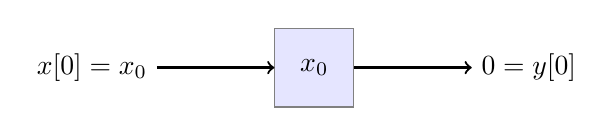
\begin{tikzpicture} [delay/.style={shape=rectangle,minimum size=1cm,draw=gray,fill=blue!10}]
	\node (delayNode) at (1,0)[delay] {$x_{0}$};
	\draw[->,thick] (-1,0) -- (delayNode.west);
	\draw[->,thick] (delayNode.east) -- (3,0);
		
	\draw (-1,0) node[anchor=east] {$x[0]=x_{0}$};
	\node at (3,0)[anchor=west] {$0=y[0]$};
\end{tikzpicture}
	
%%%%%SECOND
\vspace{0.5cm}
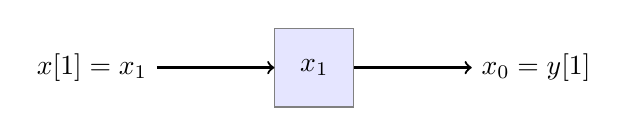
\begin{tikzpicture} [delay/.style={shape=rectangle,minimum size=1cm,draw=gray,fill=blue!10}]
	\node (delayNode) at (1,0)[delay] {$x_{1}$};
	\draw[->,thick] (-1,0) -- (delayNode.west);
	\draw[->,thick] (delayNode.east) -- (3,0);
		
	\draw (-1,0) node[anchor=east] {$x[1]=x_{1}$};
	\node at (3,0)[anchor=west] {$x_{0}=y[1]$};
\end{tikzpicture}
	
%%%%%THIRD
\vspace{0.5cm}
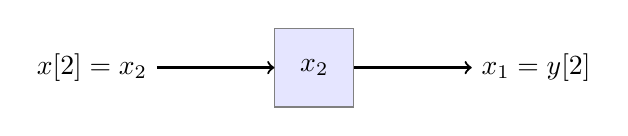
\begin{tikzpicture} [delay/.style={shape=rectangle,minimum size=1cm,draw=gray,fill=blue!10}]
	\node (delayNode) at (1,0)[delay] {$x_{2}$};
	\draw[->,thick] (-1,0) -- (delayNode.west);
	\draw[->,thick] (delayNode.east) -- (3,0);
		
	\draw (-1,0) node[anchor=east] {$x[2]=x_{2}$};
	\node at (3,0)[anchor=west] {$x_{1}=y[2]$};
\end{tikzpicture}